\problemname{Snömurskontrollant}
PO-juryn kan inte programmera. Efter fiaskot i onlinekvalet, där den trasiga domaren för problemet \href{Snömur}{https://pokval16.kattis.com/problems/pokval16.snomur} råkade ge Island vinsten med 211.58 av 100 poäng på problemet har juryn bestämt sig för att outsource:a sina domare till folk som faktiskt kan koda -- PO-finalister.

Problemet var som följer:

Sverige ska bygga en snömur, av en viss bredd $W$.
Som byggmaterial finns det ett antal snöblock som alla har höjden 1, men kan ha olika bredder.
När muren konstrueras måste varje block uppfylla följande regel: på raden under blocket,
på de två positioner blocket har sina ändpunkter, måste det ligga ett block precis till höger och vänster om punkten,
undantaget början och slutet på en rad, där det istället måste finnas en ändpunkt \emph{på varje rad} (se den vänstra, näst översta muren i Figur~\ref{fig:sample} där detta saknas på översta raden).

Det får dessutom inte finnas hålrum på samma position på två direkt efterföljande rader \emph{i muren} (den tomma raden
precis ovanför muren räknas inte).

Följande bild illustrerar några otillåtna (vänster) och tillåtna (höger) murar:

\begin{figure}[h]
	\centering
	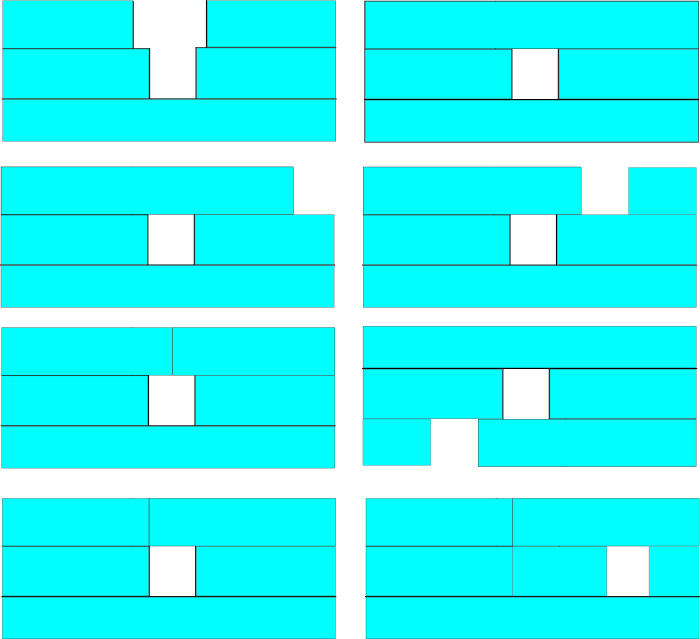
\includegraphics[width=0.7\textwidth]{mur.png}
	\caption{Ett antal otillåtna (vänster) och tillåtna (höger) murar.}
  \label{fig:sample}
\end{figure}

Givet ett förslag på hur muren ska se ut, avgör om muren är en tillåten mur.

\section*{Indata}
Den första raden innehåller två heltal $W$ och $H$ - bredden och höjden på muren.

De följande $H$ raderna beskriver raderna i muren.
Varje rad börjar med ett heltal $B \ge 1$, antalet block på raden.
Detta följs av $B$ par av heltal $P_j, L_j$, den (noll-indexerade) positionen och längden för det $j$:te blocket på raden. Dessa kommer ges i stigande $P_j$-ordning, d.v.s från vänster till höger.
Inga block kommer överlappa eller ligga utanför muren.

Raderna är givna underifrån - dvs den första raden i indata är den understa raden i muren.

Låt summan av antalet block över alla rader vara $N$.
Detta tal har gränser i poängsättnings-tabellen.

\section*{Utdata}
Du ska skriva ut \texttt{YES} om muren är tillåten, och \texttt{NO} om den inte är det.

\section*{Poängsättning}
Din lösning kommer att testas på en mängd testfallsgrupper. För att få poäng för en grupp
så måste du klara alla testfall i gruppen.

\begin{tabular}{| l | l | l | l |}
\hline
Grupp & Poängvärde & Gränser & Övrigt \\ \hline
1     & 31         & $1 \le N, W, H \le 100\,000$ & Inga hål förekommer direkt över ett annat hål \\ \hline
2     & 34         & $1 \le N, W, H \le 1,000$ & \\ \hline
3     & 35         & $1 \le N, W, H \le 100,000$ & \\ \hline
\end{tabular}

\section*{Förklaring av exempel}
De fyra första exemplen motsvarar de fyra otillåtna murarna till vänster i bilden.
De sista fyra exemplen motsvarar de fyra tillåtna murarna till höger i bilden.
